
%(BEGIN_QUESTION)
% Copyright 2010, Tony R. Kuphaldt, released under the Creative Commons Attribution License (v 1.0)
% This means you may do almost anything with this work of mine, so long as you give me proper credit

Et antimikrobielt stoff kalt {\it akrolein}, brukt for å beskytte diesel mot soppvekst, kan produseres ved å reagere propylen med damp og luft i en reaktor:

$$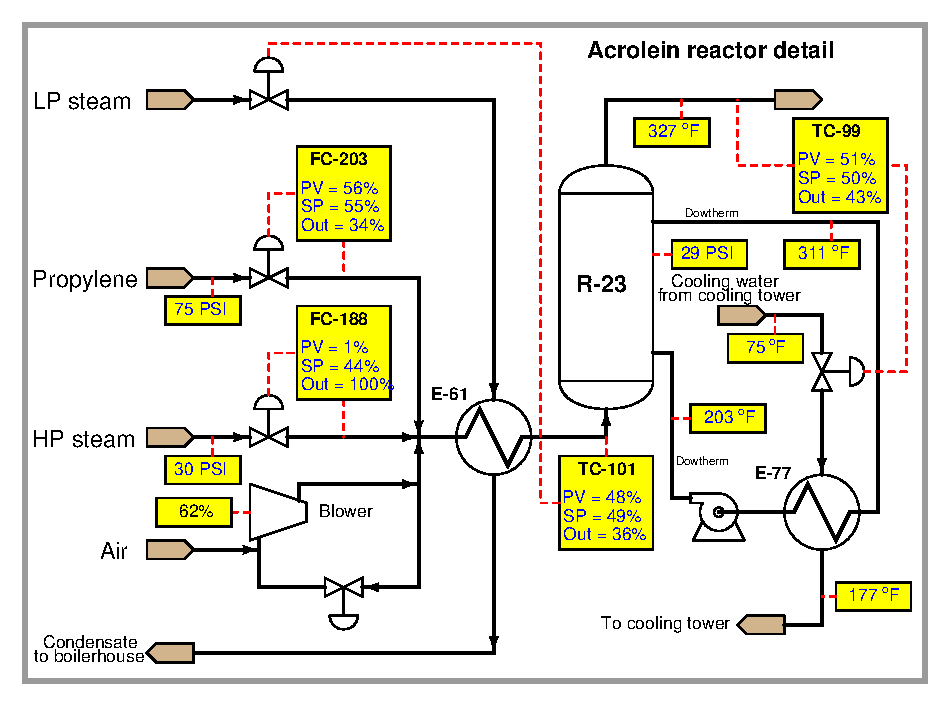
\includegraphics[width=15.5cm]{i00735x01.eps}$$

Anta at operatører ber deg feilsøke prosessen, og de viser deg denne DCS-visningen som startpunkt. Identifiser problemet, foreslå minst to mulige årsaker, og angi neste diagnostiske steg for å bekrefte årsakene.

\vskip 20pt \vbox{\hrule \hbox{\strut \vrule{} {\bf Forslag til sokratisk diskusjon} \vrule} \hrule}

\begin{itemize}
\item{} Identifiser en god feilsøkingsstrategi for slike prosessbilder, for raskt å finne {\it hvilken del av systemet} som har problemet.
\end{itemize}

\underbar{file i00735}
%(END_QUESTION)





%(BEGIN_ANSWER)

Problemet her er at damp-flowregulator FC-188 har vansker med å holde settpunkt. Mulige årsaker må utredes.

%(END_ANSWER)





%(BEGIN_NOTES)

Enten er HP-dampflow inn i reaktoren svært lav (selv om ventilen står åpen), eller transmitteren viser feilaktig for lav flow. Unormalt lavt headertrykk (30 PSI) støtter lav faktisk dampflow. Feilen ligger mest sannsynlig i dampsystemet, ikke i akroleinprosessen direkte.

Et godt neste steg er å åpne DCS-sider for dampgenerering/distribusjon. Mulig kjelhusproblem, eller en manuell dampventil kan være strupet/stengt.

%INDEX% Prosess: akroleinproduksjon
%INDEX% Prosessfeilsøking: diagnose via DCS-display

%(END_NOTES)
